\documentclass{article}
%\documentclass{amsart}
 


%%%%%%%%%%%%%%%%%%%%%%%%%%%%%%%%%%%%%%%%%%%%%%%%%%%%%%%%%%%%%%%%%%%%%%%%%%%%%%%
% language support
\usepackage{xeCJK}

% xcolor
\usepackage[dvipsnames]{xcolor}

% indentfirst
%% 添加首行缩进,两个字符,用于中文文档
%% 用于英文文档时注释以下两行
\usepackage{indentfirst}
\setlength{\parindent}{2em}

% math
\usepackage{amsfonts,amsmath,amssymb,amsthm}
\usepackage{bm}
\usepackage{mathtools}
%% define new
\newtheorem{definition}{Definition}[section]
\newtheorem{axiom}{Axiom}[section]
\newtheorem{theorem}{Theorem}[section]
\newtheorem{corollary}{Corollary}[theorem]
\newtheorem{lemma}[theorem]{Lemma}
\newtheorem*{remark}{Remark}
\newtheorem*{exercise}{Exercise}

% hyperref
\usepackage{hyperref}
\hypersetup{
	colorlinks=true,
	linkcolor=blue,
	pdftitle={SELinux},
}

% acronym
\usepackage[acronym]{glossaries-extra}
\setabbreviationstyle[acronym]{long-short}
\makeglossaries
\newacronym{selinux}{SELinux}{Security-Enhanced Linux}
\newacronym{dac}{DAC}{Dictionary Access Control}
\newacronym{mac}{MAC}{Mandatory Access Control}
\newacronym{dbms}{DBMS}{Database Management system}
% tcolorbox
\usepackage{tcolorbox}

% geometry
%% it's useful to adjust page margins and line spacing.
% \usepackage[left=2cm, right=2cm, top=1.54cm, bottom=1cm]{geometry}
\usepackage[margin=2.5cm]{geometry}

% fancyhdr
%% fancyhdr 需要放在 geometry 后面
\usepackage{fancyhdr}
\pagestyle{fancy}
\fancyhead[R]{\leftmark} % 设置右页眉为章节标题


% setspace
%% a simple way of changing line spacing
%% e.g. for 1.5x line spacing
% \usepackage[onehalfspacing]{setspace}
%% [doublespacing] for 2x line spacing

% siunitx
\usepackage{siunitx}

% graphicx
%% include the graphics
%% e.g. scale the image to 80% of the text width
% \includegraphics[width=0.8\textwidth]{figure.eps}
%% e.g. fix the hight and width of a figure
%% [width=2cm, height=5cm]
%% e.g. rotate 90 degrees
%% [angle=90]
%% set the default path
% \graphicspath{{./figures}{./additionalFigures}}

% biblatex
% \usepackage{biblatex}

% lineno
%% 每行数字序列
% \usepackage{lineno}
% \linenumbers


\newcommand{\bsl}{\texttt{\symbol{92}}}



\title{数据中心气流组织}
\author{郑海腾}
\date{\today}

\begin{document}
\maketitle
\tableofcontents

\newpage
\begin{abstract}
	随着数字社会的发展,为满足信息化发展的需要,支撑数据业务。大量且数据中心得以建设。
数据中心的规模也不断的扩大。绝大多数的数据中心在建设时都采用的地板送风的方法。为使得
服务器运行稳定,减少数据中心能耗,提高制冷效果,本文综合介绍了各种气流组织对数据中心热性能的影响。

\noindent \textbf{关键字:} 数据中心;气流组织;地板送风
\end{abstract}

\section{引言}
\subsection{研究背景}
随着近些年来计算机技术的飞快发展,互联网和物联网在带来巨大用户量的同时产生了海量的数据。
作为支持信息化建设的基础设施,数据中心承担着重要的作用。但与此同时,数据中心规模的逐渐
扩大,其机架数量屡屡突破新高~\cite{1}。与之而来的能耗问题逐步严重,如何降低能耗对数据
中心的建设及其重要。

\subsection{国内现状}
据相关数据统计,在 2020 年,我国数据中心的年用电量已经达到了$\qty{2500}{\text{亿}~\kWh} $,占据了全国用电量的 3\% 以上~\cite{2},在 2021 年,我国数据中心的年用电量达到了$\qty{2166}{\text{亿}~\kWh}$,占据全国用电量 2.6\%~\cite{3}。伴随着深度
学习技术进步,层出不穷的大模型训练要求更多的数据中心提供更多的算力支持,许多新能源车企也开始搭建数据中心用于智能驾驶模型训练,三大运营商也开始深入开展数据中心建设~\cite{7},可见数据中心规模将逐渐增大,其能耗增加也将快速增长~\cite{4}。很显然,科技的迅速发展需要更多的数据中心提供支持,但其伴随的能耗问题十分严重,降低能耗对于数据中心十分重要。

\subsection{国外现状}
据相关数据表明,英国数据中心的用电量占据着英国全国用电总量的 1.5\%,且其增长速度超过 15\%~\cite{5}。
数据中心的能耗组成主要包括 IT 设备、空调冷却系统、UPS 供配电系统和照明系统四部份。
美国数据中心的数据表明其能耗的 40\% 由冷却系统产生~\cite{6}。

\subsection{气流组织}
数据中心气流组织是指对其各个单元机房内的气流运动进行组织与管理,管理分配冷却系统的冷空气并回收热空气,促进机房内部设备热量传递,保障设备满足热环境需求。

数据中心的能耗优化可以从结构、布局和气流组织等方面进行。数据中心密集度高,为有效消除某些局部热点,可对机房内的气流组织进行优化。如图~\ref{F:1} 所示,机柜大多同面相对,采用地板送风的形式。相比较与顶部送风的方法,地板送风的方式传输的气流均匀,噪音也更小~\cite{8}。

\begin{figure}[htbp]
	\centering
	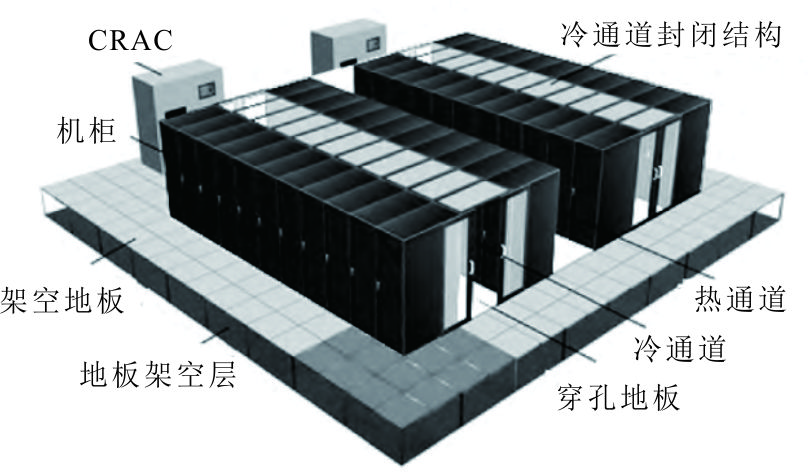
\includegraphics[width=\textwidth]{figure/figure_1.jpg}
	\caption{地下送风封闭式数据中心模型}
	\label{F:1}
\end{figure}

Shrivastava~\cite{9} 通过对两种送气形式的研究,对比得出了地板送风的气流组织效果较好。RR~SCHMIDT~\cite{10} 也同样进行了对比研究,得到地板下送风的形式有利于供气均匀。许陆顺~\cite{11} 等人通过对数据中心冷通道导流结构~\ref{F:2} 的研究,得到合理和导流结构使得数据中心的温度场和速度场均匀,避免积热。杨力芝等人~\cite{12} 使用 CFD 的方法测试地板送风方式对数据中心热环境的影响,得到地板下送风冷通道封闭方式冷气流利用更充分。李婷婷等人~\cite{13} 使用模拟软件对比的两种送风方式产生的温度场和速度场,发现不受开孔率影响的机架地板送风形式冷量利用率更高。陈修敏等人~\cite{14} 模拟发现了机房局部气流不通畅,存在局部热点。

\begin{figure}[htbp]
	\centering
	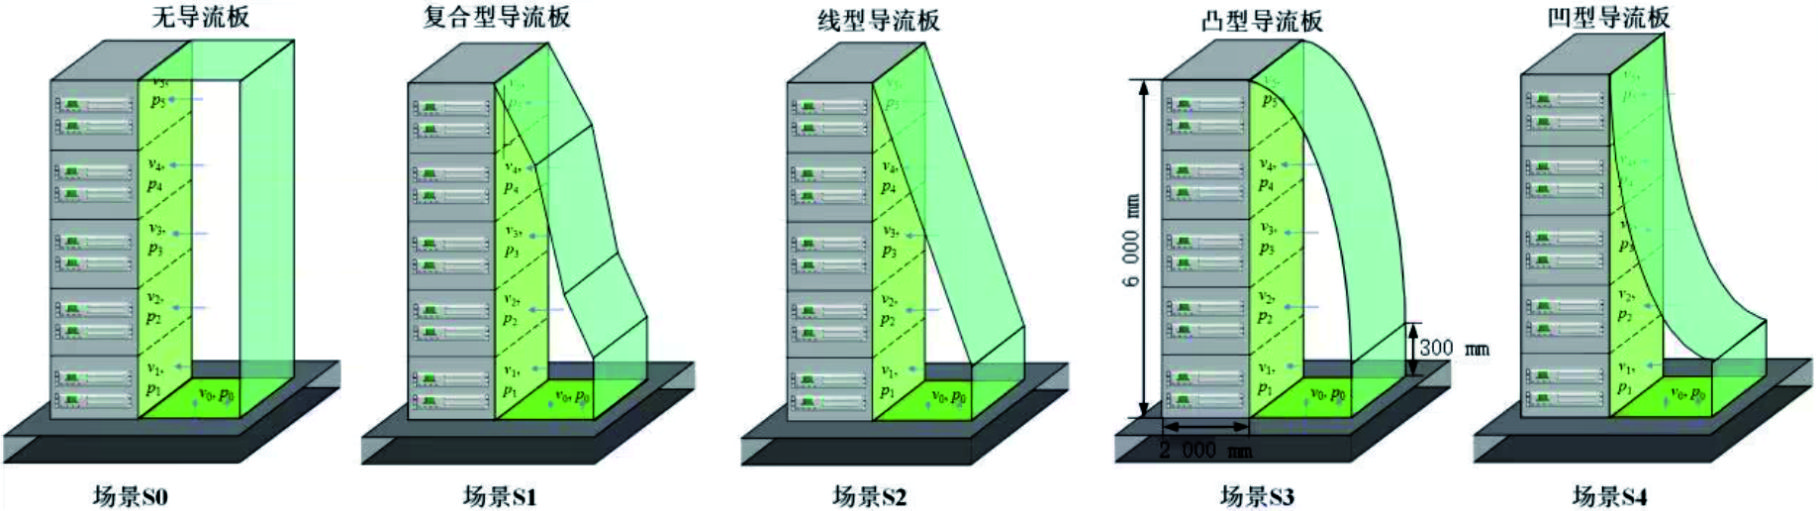
\includegraphics[width=0.7\textwidth]{figure/figure_2.jpg}
	\caption{导流板示意图}
	\label{F:2}
\end{figure}

\newpage
\noindent 气流组合有三点核心问题~\cite{16}:
\begin{itemize}
	\item 冷热空气掺杂
	\item 热空气再循环
	\item 冷空气旁通
\end{itemize}

\section{送风形式}
主要的三种典型气流组织为风管上送风、地板下送风和列间空调前送后回。张学娇~\cite{17} 对三种
送风方式在机房环境和空调系统参数一定时进行比较,得到列间送风比其他两种送风方式的冷量利用率更高。

\subsection{风管上送风}
由于需要安装风管,该方式对房间楼层净高有一定要求,增加数据中心的建设成本。风管上送风的形式容易造成局部热堆积~\cite{15}。此外,风管上送风在建造完成后不易再次调整,还存在噪音大(往往达到 70 dB 以上~\cite{19})等缺点。由于送风是从各个风口出来,送风不均匀。

此种形式的送风主要存在于老旧机房,在各项指标要求高的现代大机房中已被淘汰。
\subsection{地板下送风}
地板下送风广泛被当前数据中心采用。其施工简单,可隐藏各种管道线缆,还可后期随时调整地板开孔率。申佳惠~\cite{21} 指出地板下送风通过静压和地板的隔离作用可以将冷空气输送到$\qty{15}{\m}-\qty{20}{\m} $的地方,但由于出风口的阻力损失,风机需要克服机外余压大。

\begin{figure}[htbp]
	\centering
	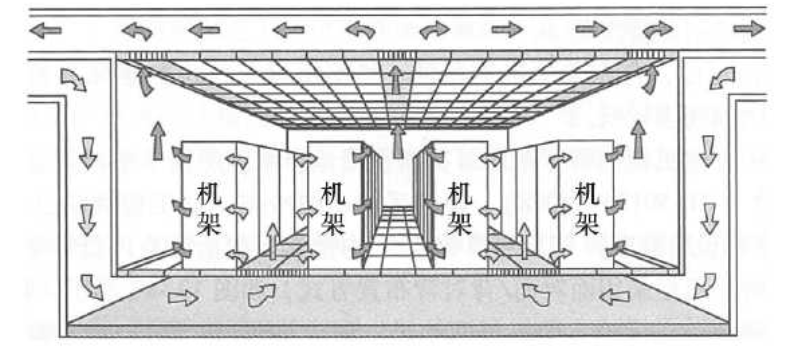
\includegraphics[width=0.7\textwidth]{figure/figure_3.png}
	\caption{地板下送风示意图}
	\label{F:3}
\end{figure}

\subsection{列间空调送风}
作为一种新的制冷方式,其有效缩短了出风口至机架的距离。许坚强~\cite{18} 指出列间空调采取气流测送后回的方式时,能有效避免两侧风阻大、送风量小的问题,并能减少气流短路和混合现象,提高冷量利用效率。严瀚~\cite{20} 指出列间送风摆脱了长距离送风射流的损失,减少紊流和扰流。申佳惠~\cite{21} 指出列间空调可结合封闭通道形成冷池效应,实现备用制冷效果。

\begin{figure}[htbp]
	\centering
	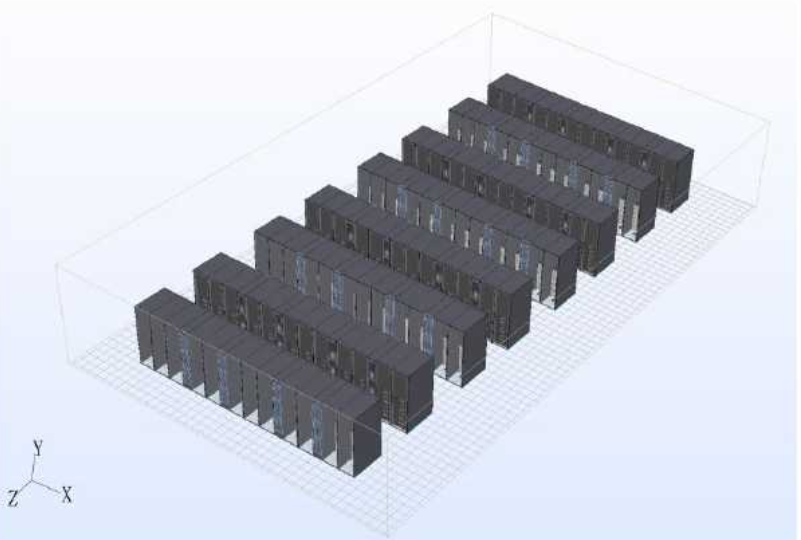
\includegraphics[width=0.7\textwidth]{figure/figure_4.png}
	\caption{列间送风模型图}
	\label{F:4}
\end{figure}

\newpage
\section{结论}
本文针对数据中心的能耗问题,叙述了不同的气流形式有各自的特点,分析并利用它们的特点可以达到提高能效、减少能耗的目的。
\begin{itemize}
	\item CFD 模拟可以将气流组织于数据中心这个黑箱建立联系,分析各气流组织的特点。以便于优化数据中心的建设。
	\item 分析各送风方式的影响,通过冷通道送风实测可发现存在的热堆积点,后续可针对该点进行优化。
	\item 末端空调的运行方案影响冷通道的流速场,而速度场决定压力场的分布,可分析气流是否均匀,减少冷量损失。以改善数据中心的热环境。
\end{itemize}

\newpage
\printbibliography

\end{document}
